\chapter{太阳系}\label{ch:g4:solar-system}

你知道吗，地球每年绕太阳公转一圈。但它
是独自旅行吗？晴朗的夜晚抬头看看，在固定的
星星之间，有几颗明亮的光点每周都在缓慢移动。古人
称它们为“游星”；我们称它们为行星——它们和地球
一样，环绕同一颗太阳运行。

\section{一颗恒星，八颗行星}

\begin{definition}[恒星]\label{def:g4:solar-system:star}
\emph{恒星}\index{恒星}是一个巨大的炽热发光物质球，
能够自己发光——是真正的光源。太阳是
一颗恒星：离我们很近，足以温暖我们的脸庞。（夜晚的其他
恒星，明年将有属于它们自己的一章。）
\end{definition}

\begin{definition}[行星]\label{def:g4:solar-system:planet}
\emph{行星}\index{行星}是一个又大又圆、绕恒星运行的天体，
自身不发光——我们看到行星，就像看到月球一样，
是因为它们反射了太阳光。地球
是一颗行星。
\end{definition}

\begin{definition}[太阳系]\label{def:g4:solar-system:family}
\emph{太阳系}\index{太阳系}是太阳以及所有绕它运行的天体，
包括八颗行星——按顺序为水星、金星、地球、火星、木星、土星、
天王星、海王星——外加它们的卫星，以及许多较小的岩石
和冰块。
\end{definition}

\begin{omfigure}
\begin{tikzpicture}[scale=0.85]
  % the Sun, anchored in the corner
  \fill[omThm] (0,0) -- (0.65,0) arc (0:40:0.65) -- cycle;
  \node[below, font=\small] at (0.45,-0.95) {太阳};
  % one generous arc of each orbit
  \foreach \r in {1.3, 2.1, 2.9, 3.7, 5.2, 6.9, 8.5, 10.1} {
    \draw[dashed, omExo] (\r,0) arc (0:40:\r);
  }
  % the planets, labels staggered in two rows
  \foreach \r/\name in {1.3/水星, 2.9/地球, 5.2/木星,
      8.5/天王星} {
    \fill[omDef] (\r,0) circle (0.11);
    \node[below, font=\footnotesize] at (\r,-0.18) {\name};
  }
  \foreach \r/\name in {2.1/金星, 3.7/火星, 6.9/土星,
      10.1/海王星} {
    \fill[omDef] (\r,0) circle (0.11);
    \draw[omExo, very thin] (\r,-0.18) -- (\r,-0.72);
    \node[below, font=\footnotesize] at (\r,-0.75) {\name};
  }
\end{tikzpicture}

{\small 太阳及其八颗行星，按顺序排列——这里画得紧紧挨在一起，
但实际上每条轨道都远远
位于前一条轨道之外。}
\end{omfigure}

\begin{proposition}[行星的运行规律]\label{prop:g4:solar-system:habits}
行星运行很有规律：每一颗都沿着自己
近似圆形的轨道绕太阳运行，它们的绕行方向都相同，
所有轨道几乎位于同一平面内，就像
画在同一张桌面上的圆环。行星的轨道离太阳越远，
绕行一周所用的时间就越长：水星用 $88$ 天，地球用一年，
最远的海王星则需要 $165$ 年。
\end{proposition}

\begin{example}[岩质行星与气态巨行星]\label{ex:g4:solar-system:kinds}
水星、金星、地球、火星这四颗内侧行星，都是
又小又坚实的岩石球：是你可以站上去的世界。外侧的四颗
木星、土星、天王星、海王星——是
\emph{巨行星}：主要由浓厚气体构成的巨大球体，
完全没有可以站立的地面。最大的木星
能装下一千多个地球；土星有著名的明亮光环，
由无数细小的冰块组成，环绕土星，宛如一群微型卫星。
\end{example}

\begin{omfigure}
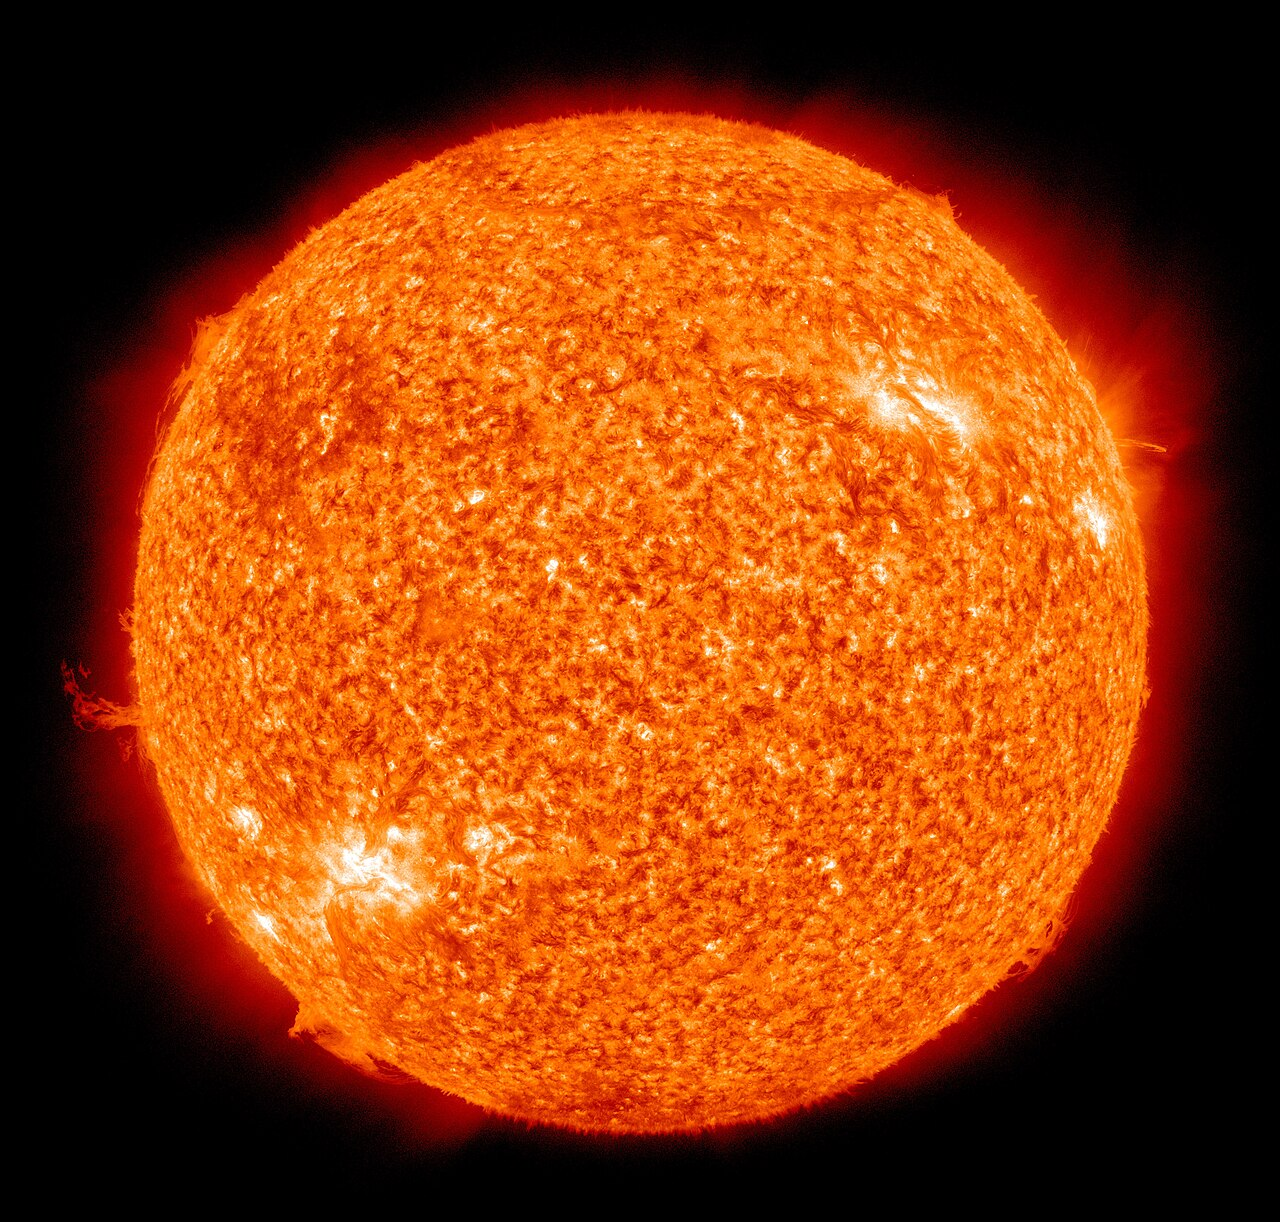
\includegraphics[height=3.1cm]{images/book1/sun-sdo.jpg}

{\small 太阳，我们的恒星}

\medskip
\begin{tabular}{cccc}
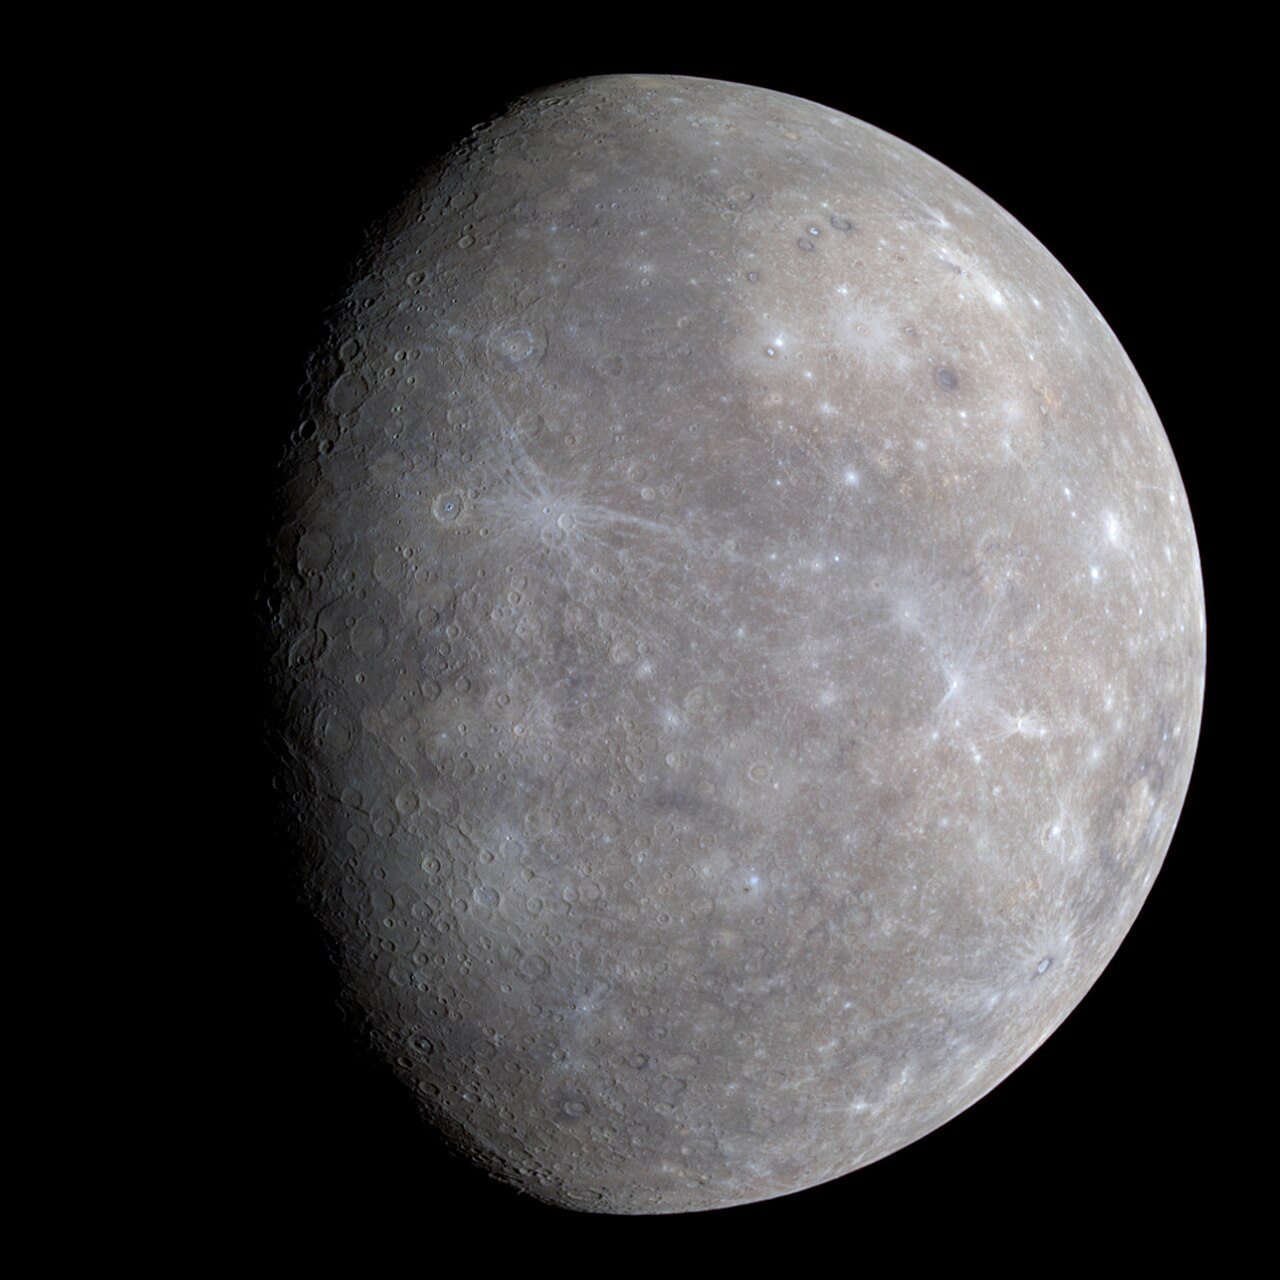
\includegraphics[height=1.75cm]{images/book1/mercury.jpg} &
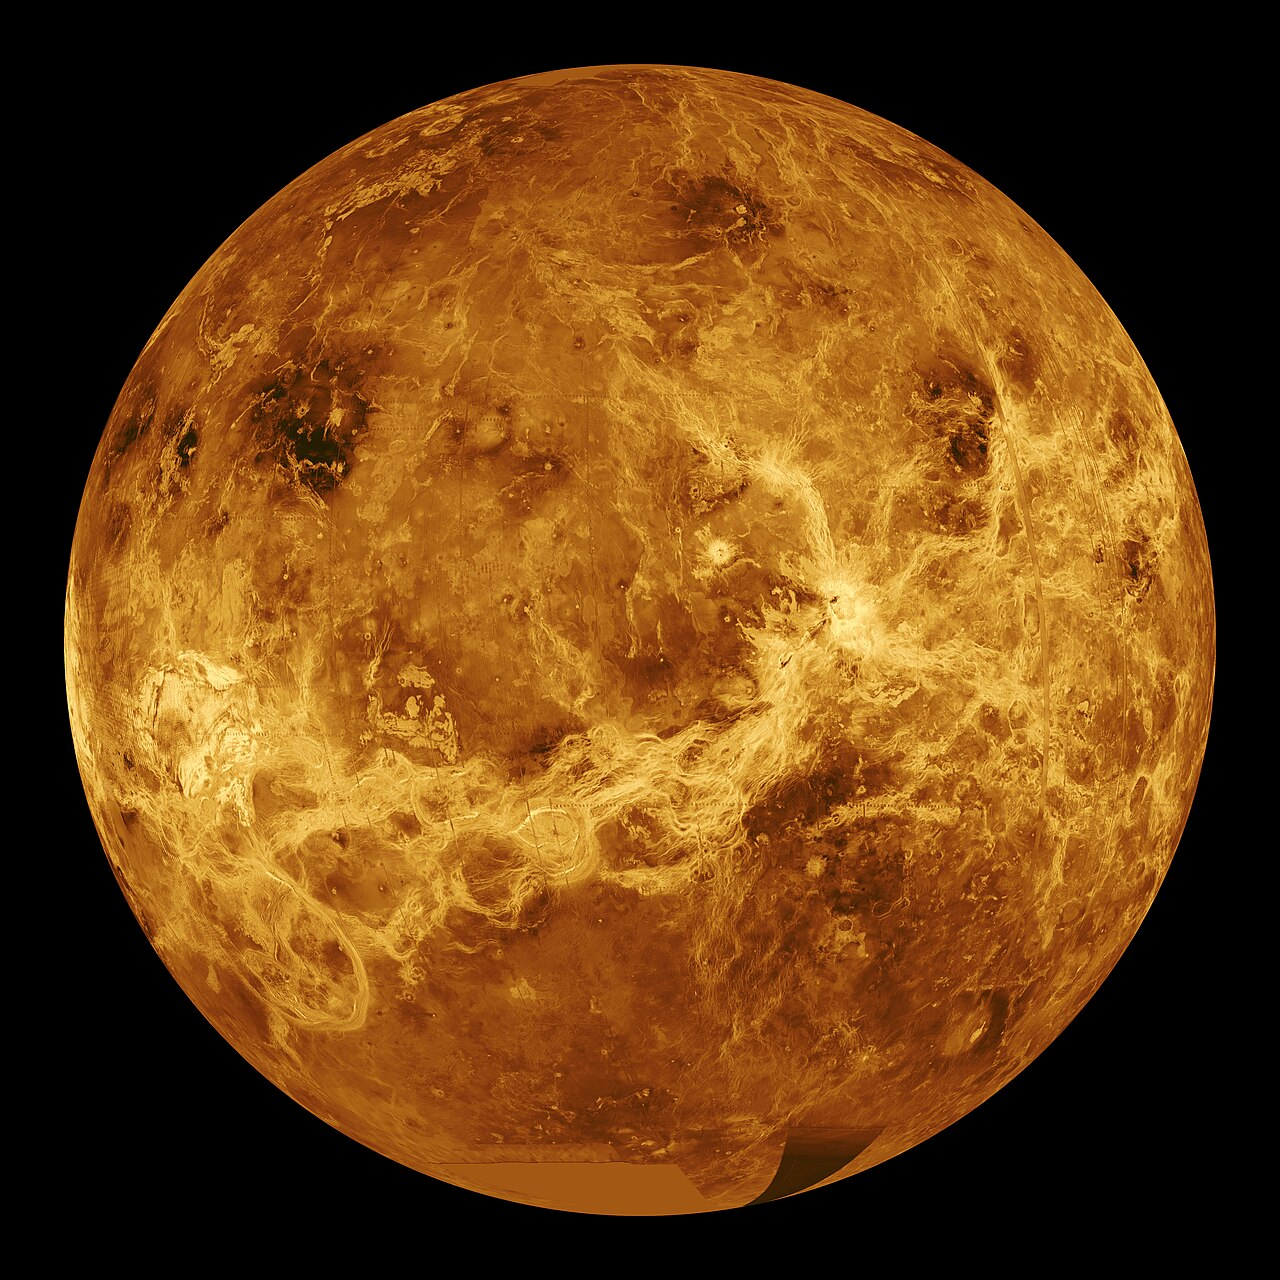
\includegraphics[height=1.75cm]{images/book1/venus.jpg} &
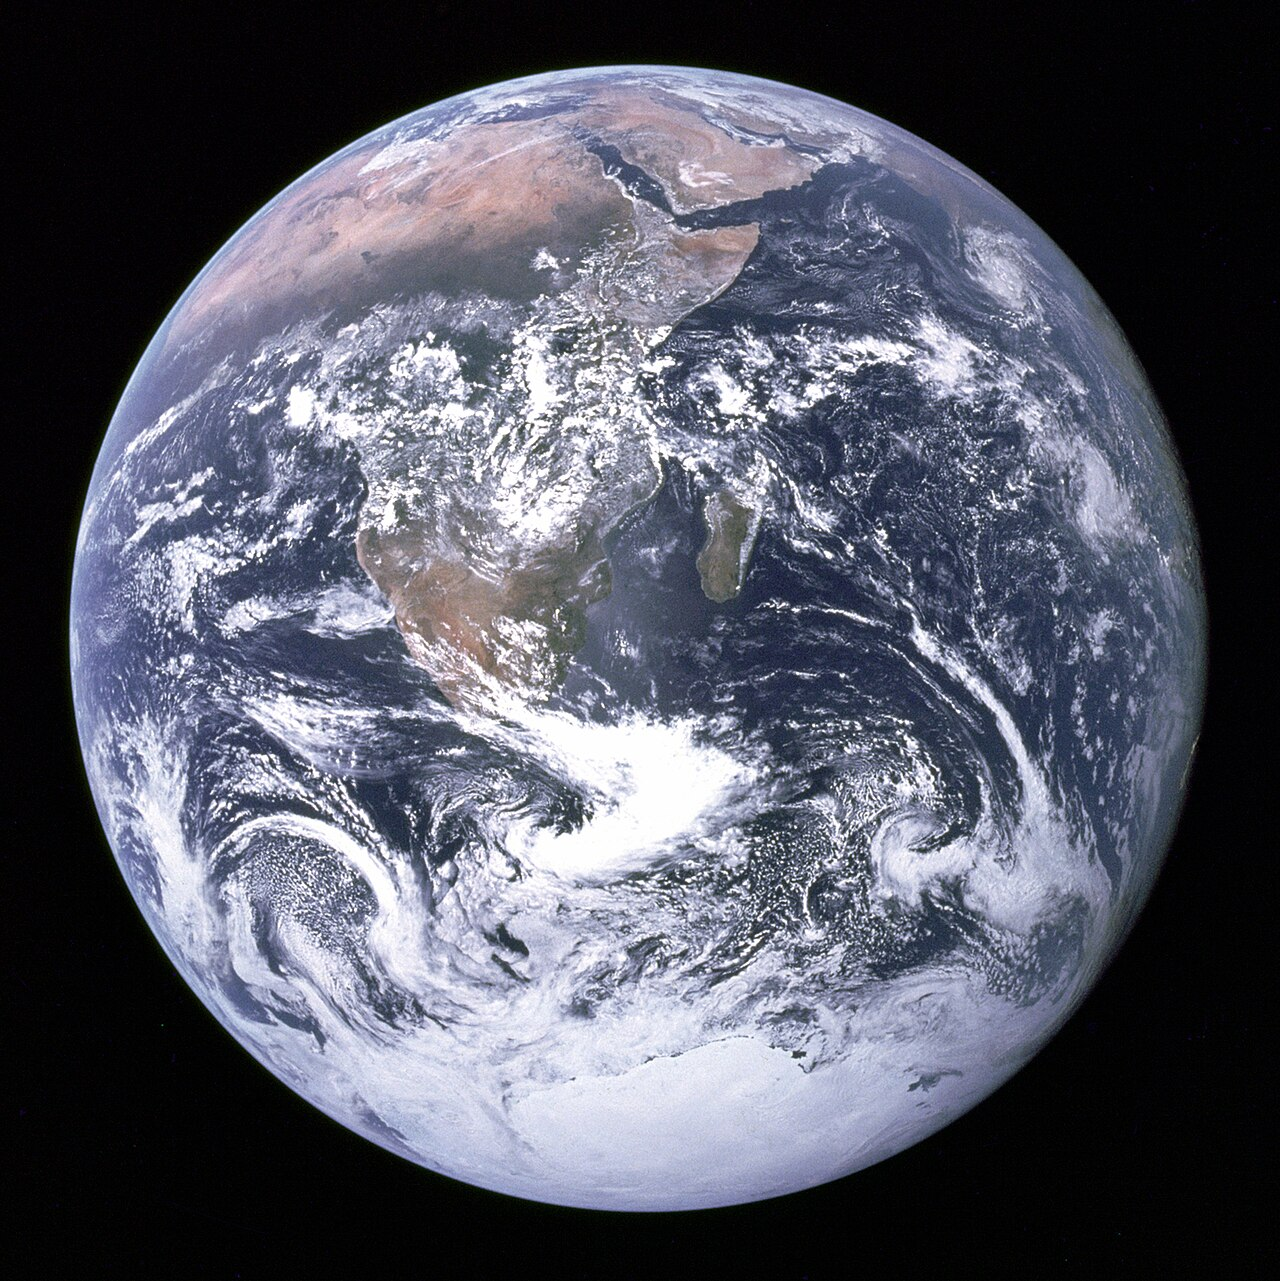
\includegraphics[height=1.75cm]{images/book1/earth.jpg} &
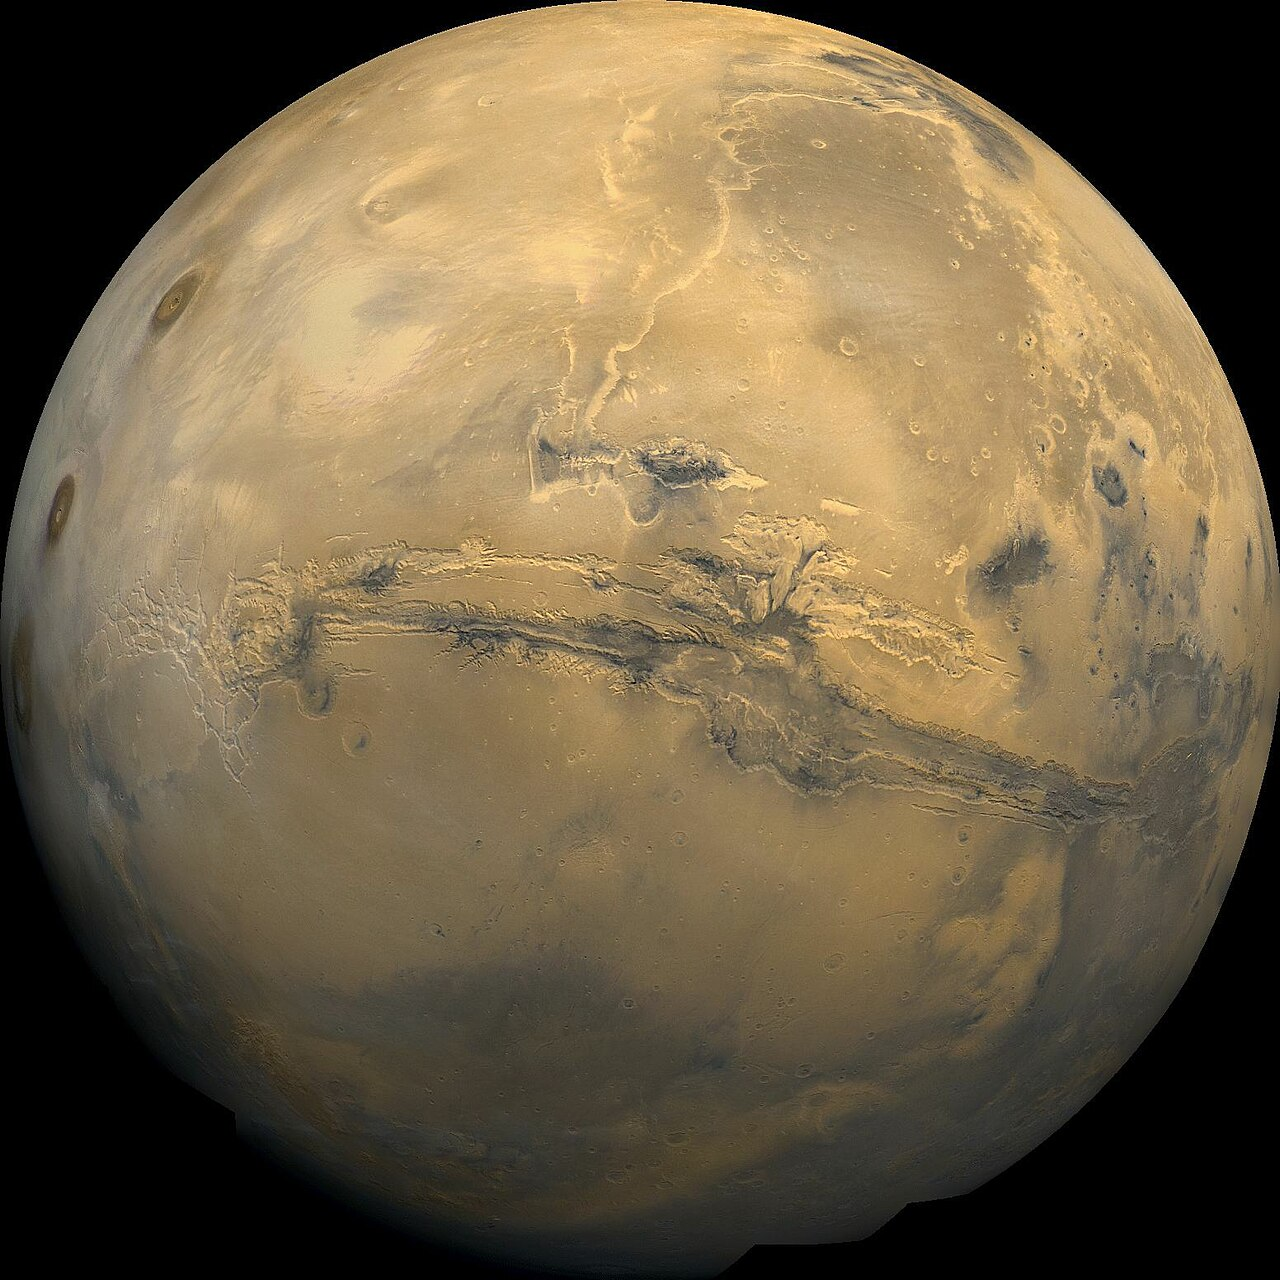
\includegraphics[height=1.75cm]{images/book1/mars.jpg} \\
{\footnotesize 水星} & {\footnotesize 金星} &
{\footnotesize 地球} & {\footnotesize 火星} \\[4pt]
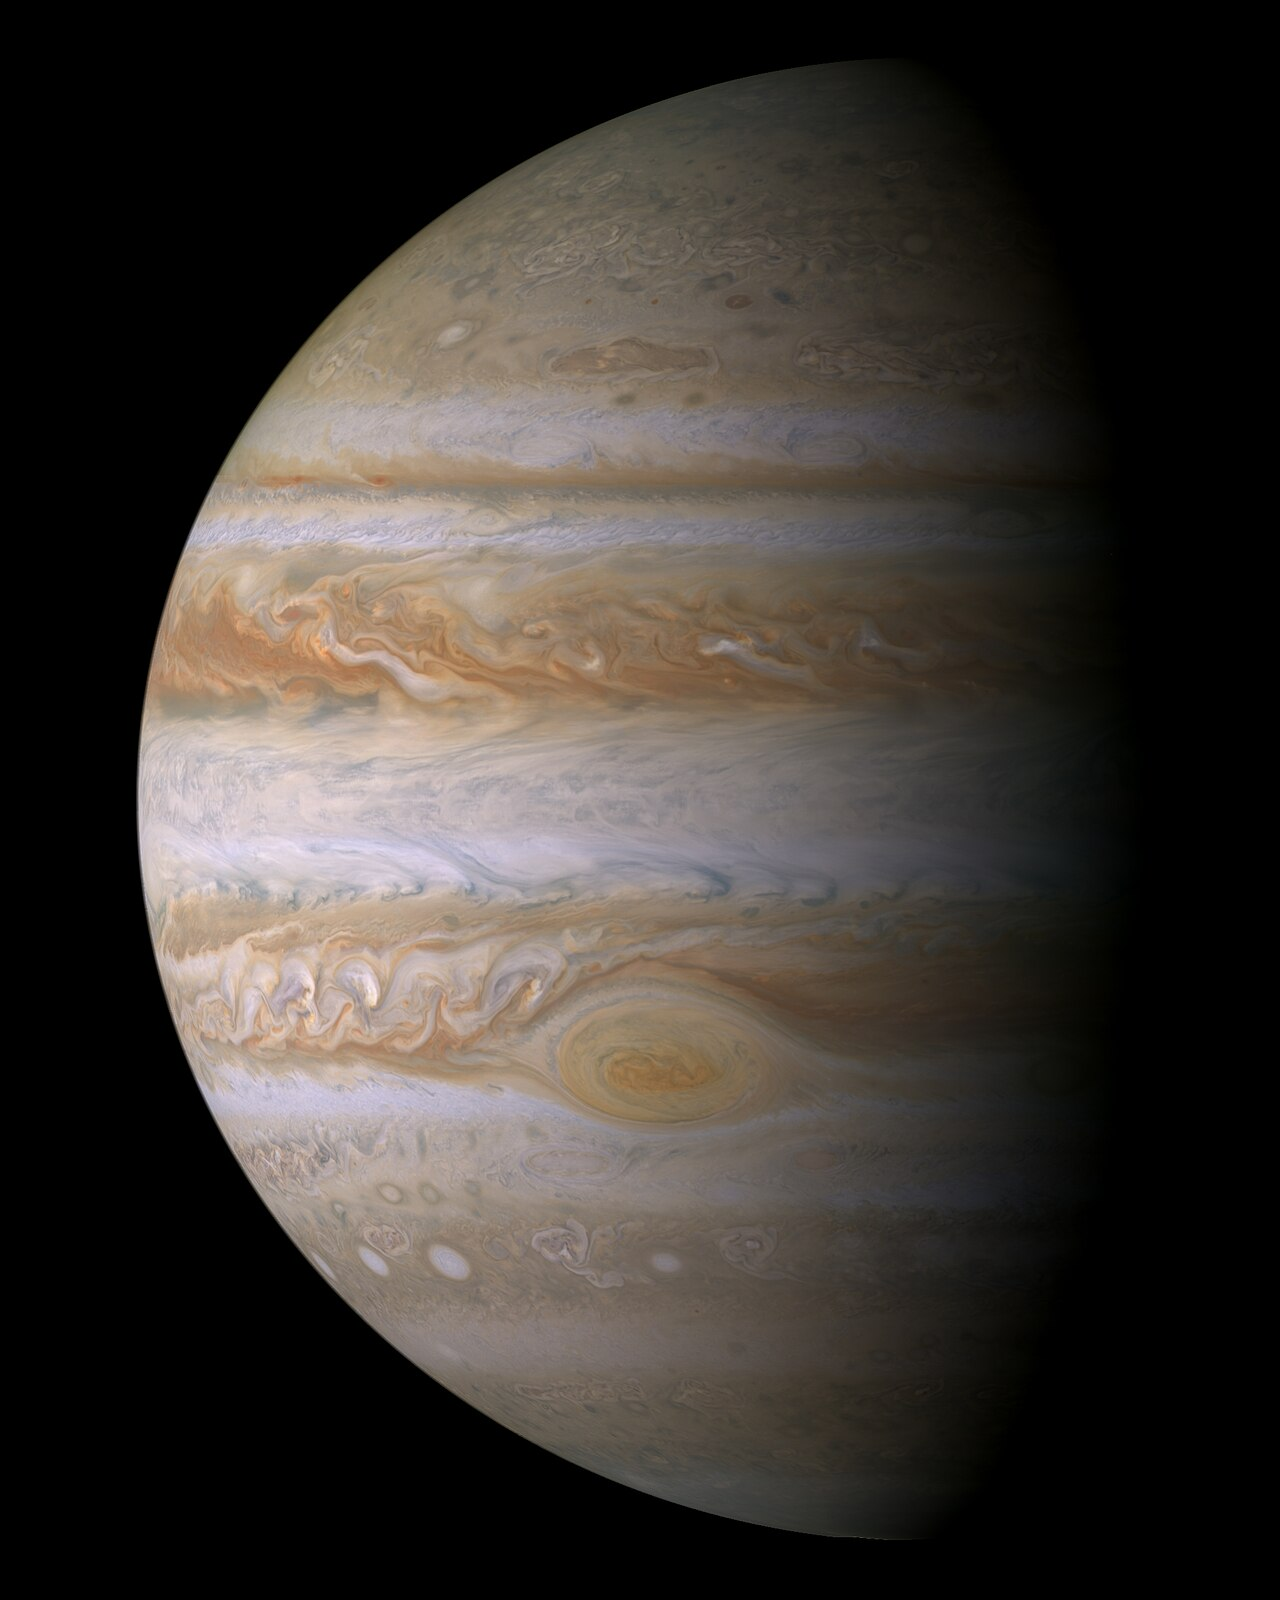
\includegraphics[height=1.75cm]{images/book1/jupiter.jpg} &
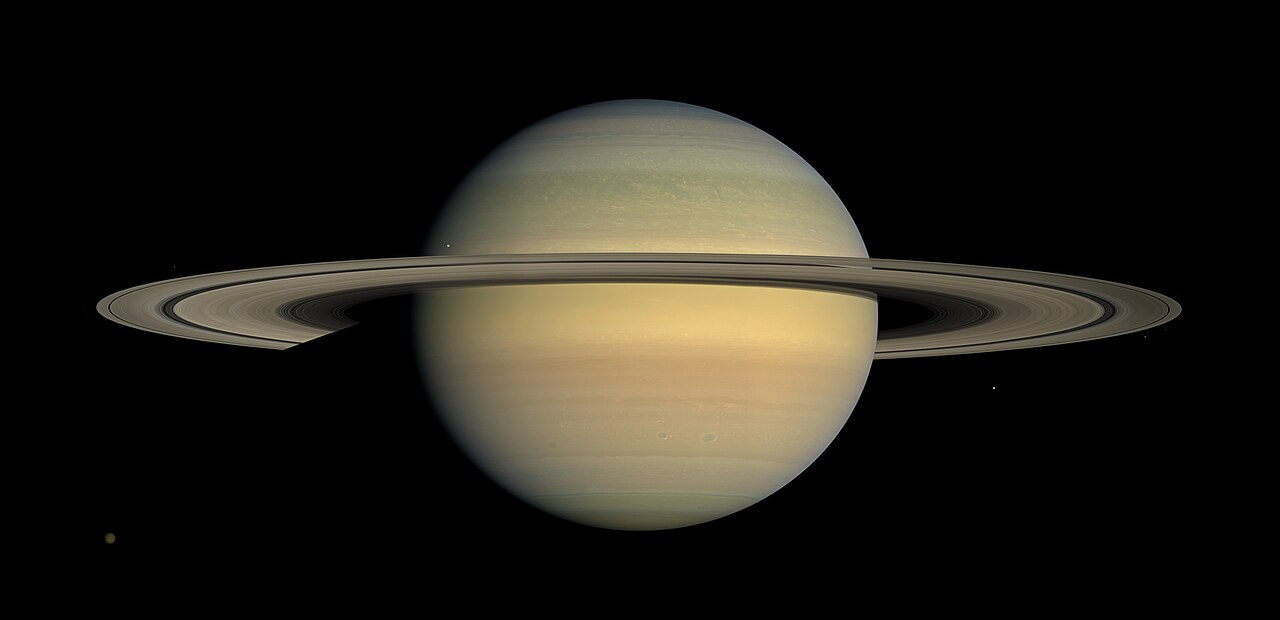
\includegraphics[height=1.75cm]{images/book1/saturn.jpg} &
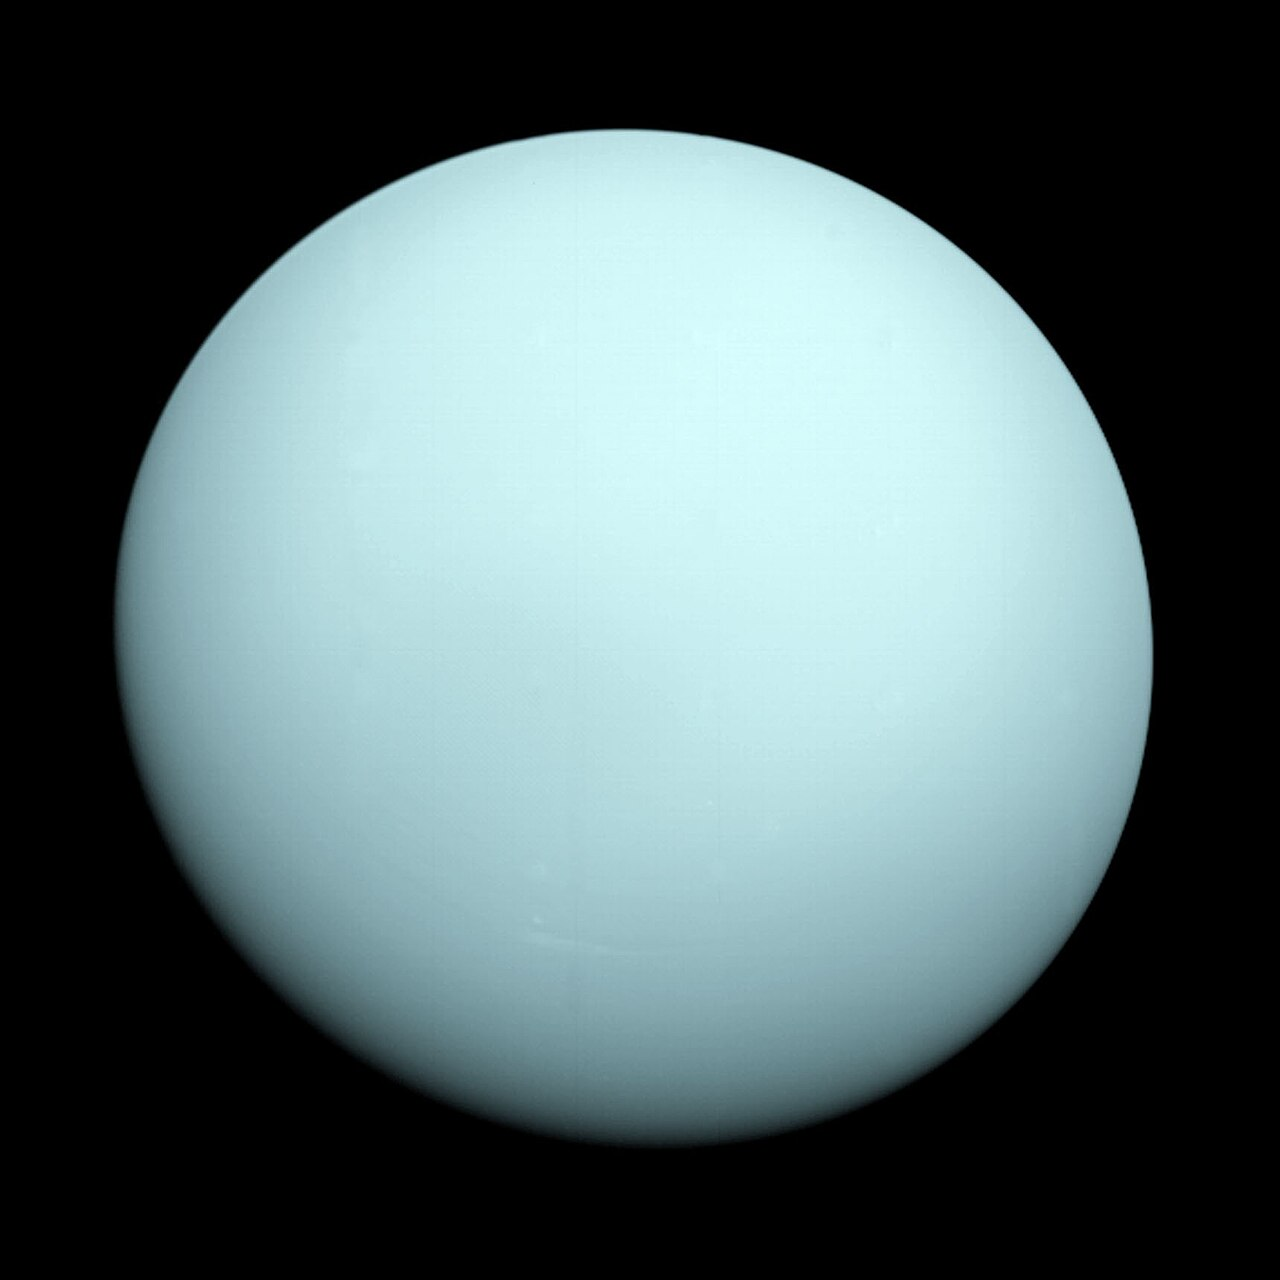
\includegraphics[height=1.75cm]{images/book1/uranus.jpg} &
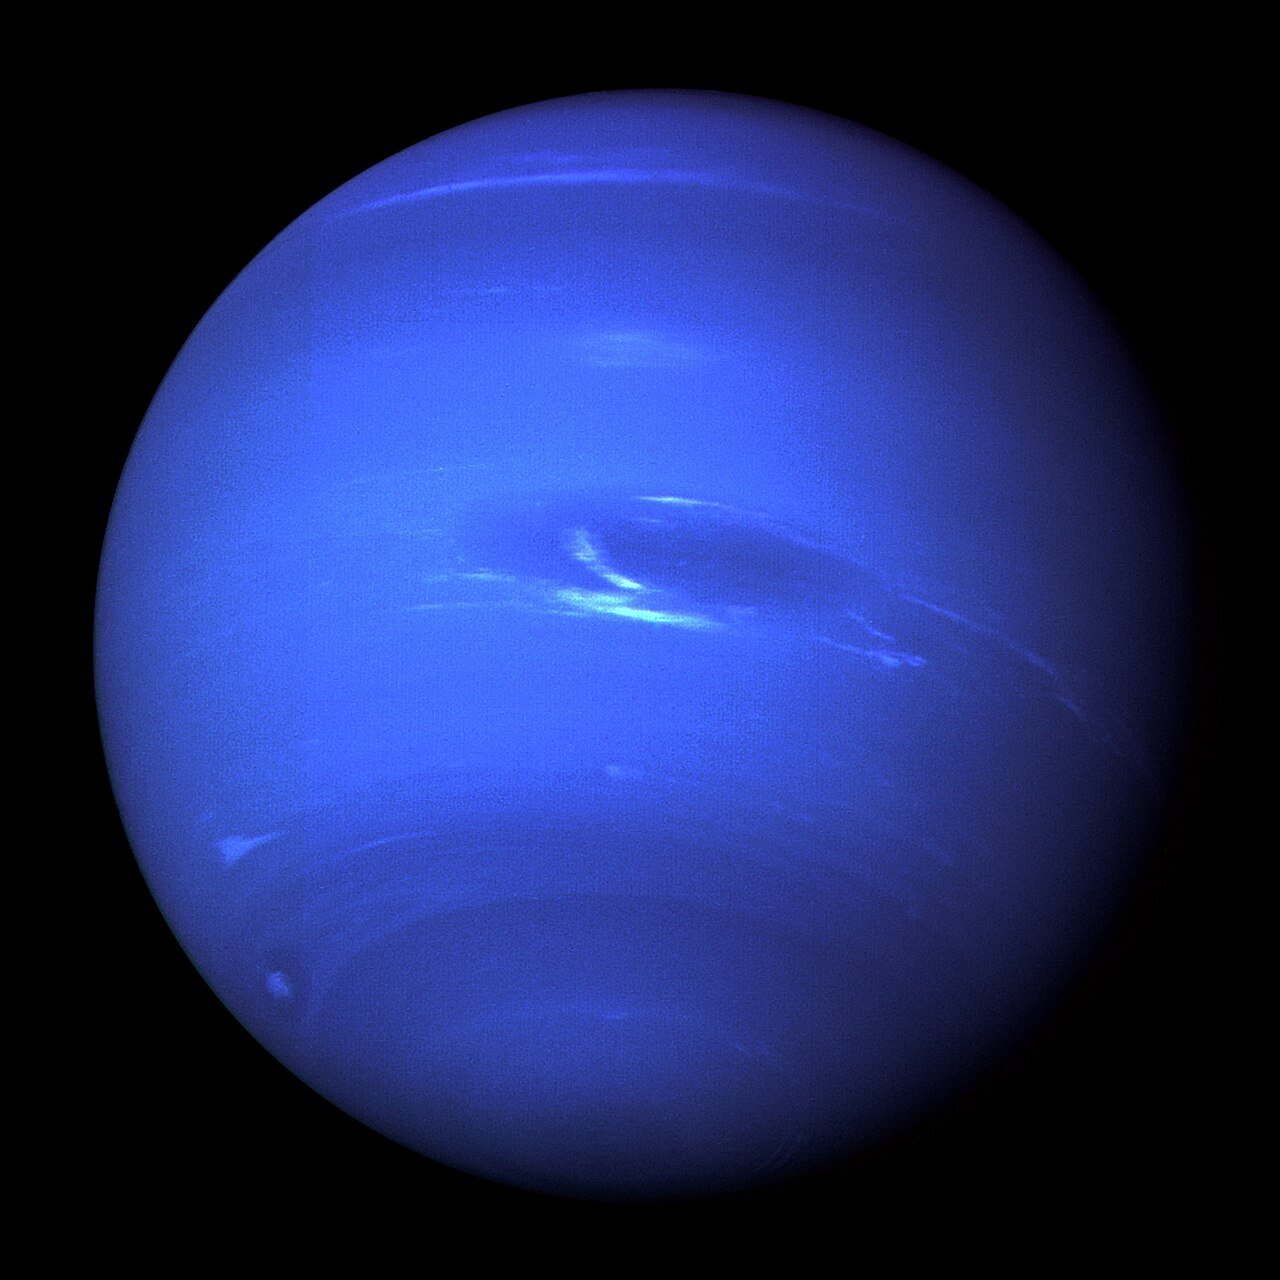
\includegraphics[height=1.75cm]{images/book1/neptune.jpg} \\
{\footnotesize 木星} & {\footnotesize 土星} &
{\footnotesize 天王星} & {\footnotesize 海王星}
\end{tabular}

{\small 太阳及其八颗行星的真实面貌，
由太空探测器拍摄（大小与距离未按比例绘制；
金星以雷达图显示——其云层遮住了地表）。
\emph{照片：NASA（公有领域）。}}
\end{omfigure}

\begin{example}[月球不是行星]\label{ex:g4:solar-system:moons}
我们的月球绕的是\emph{地球}，而不直接绕太阳运行——所以它
不是行星，而是\emph{卫星}，即行星的伴随天体。其他
行星也有自己的卫星：火星有两颗小卫星，木星
和土星各有数十颗。卫星属于它的行星，
而行星则属于太阳。
\end{example}

\section{远有多远}

\begin{method}[太阳系的比例模型]\label{met:g4:solar-system:model}
行星之间的距离大得惊人——以百万
千米计。为了感受这些距离，可在公园里搭建一个太阳系的比例模型，
将所有大小与距离按同一比例缩小：
\begin{enumerate}
  \item 让太阳成为放在大门口的一个足球；
  \item 然后地球是一粒胡椒粒——为了公平地放置它，
        从足球处起走约 $30$ 大步；
  \item 水星是一个针头，离足球约 $12$ 步；
        木星是一颗弹珠，约 $150$ 步；海王星是一颗小珠子，
        约 $900$ 步——将近一千米远！
\end{enumerate}
走一走，亲身感受图画无法展示的东西：太阳系几乎全是空旷的空间，
其中的小小世界彼此相距极远。在这个模型中，
一大步约代表真实空间中的五百万千米。
\end{method}

\begin{omfigure}
\begin{tikzpicture}[scale=0.85]
  \draw[-Stealth, thick] (0,0) -- (11.2,0);
  \fill[omThm] (0.5,0) circle (0.3);
  \node[below, font=\footnotesize] at (0.5,-0.42) {足球};
  \fill[omDef] (1.6,0) circle (0.05);
  \draw[omExo, very thin] (1.6,-0.18) -- (1.6,-0.85);
  \node[below, font=\footnotesize] at (1.6,-0.88) {针头};
  \fill[omDef] (3.2,0) circle (0.08);
  \node[below, font=\footnotesize] at (3.2,-0.35) {胡椒粒（地球）};
  \fill[omDef] (6.0,0) circle (0.16);
  \draw[omExo, very thin] (6.0,-0.24) -- (6.0,-0.85);
  \node[below, font=\footnotesize] at (6.0,-0.88) {弹珠（木星）};
  \fill[omDef] (10.6,0) circle (0.1);
  \node[below, font=\footnotesize] at (10.6,-0.38) {小珠子（海王星）};
  \node[above, font=\small] at (5.6,0.5)
    {$12$ 步，$30$ 步，$150$ 步，$900$ 步\dots};
\end{tikzpicture}

{\small 比例模型：把太阳缩成一个足球，整个太阳系
刚好能放进一座公园——勉强够用。}
\end{omfigure}

\begin{example}[天空中的漫游者]\label{ex:g4:solar-system:wanderers}
金星常常是傍晚最先出现的“星星”，在日落后的西方天空
熠熠生辉——它之所以如此明亮，是因为它是我们最近的
邻居，外面包裹着白色云层，能慷慨地把阳光反射回来。
火星发出微弱的橙色光；木星和土星则明亮而稳定。
若连续几周对照背景中的恒星观察其中一颗，
恒星位置不变，它却会慢慢挪动——正是这种“漫游”，
赋予了行星古老的名字。
\end{example}

\begin{remark}[一幅旧图的重绘]\label{rem:g4:solar-system:history}
长期以来，人们把地球放在万物的中心，
太阳、月球和行星都绕着我们转。细心的观测者
对行星的漫游进行观察后发现，这幅图景已摇摇欲坠——行星
有时会\emph{逆行}一段时间，这难以用地球居于中心来解释。
地球居于正中。你刚学过的日心图景
能简单地解释这些漫游，它也是人类接受过的
最大胆的思想之一：我们的家园并非
宇宙的中心——它是离太阳第三近的行星。
\end{remark}

\section{练习}

\begin{exercise}[$\star$]\label{exo:g4:solar-system:1}
恒星与行星有什么区别？下面哪一个是
太阳？哪一个是地球？
\end{exercise}

\begin{exercise}[$\star$]\label{exo:g4:solar-system:2}
按离太阳由近到远的顺序，背出八颗行星。哪一颗是我们的？
\end{exercise}

\begin{exercise}[$\star$]\label{exo:g4:solar-system:3}
哪些行星小而由岩石构成？哪些是气态巨行星？
说出最大的那颗，以及拥有著名光环的那颗。
\end{exercise}

\begin{exercise}[$\star$]\label{exo:g4:solar-system:4}
月球为什么不算行星？它绕的是什么？
\end{exercise}

\begin{exercise}[$\star$]\label{exo:g4:solar-system:5}
水星绕太阳一圈需要 $88$ 天，地球需要 $365$ 天，海王星需要
$165$ 年。这些数字说明了行星的什么规律？
\end{exercise}

\begin{exercise}[$\star$]\label{exo:g4:solar-system:6}
在公园比例模型中，什么代表太阳？地球离它
有多少步远？按空间计算，太阳系的几乎全部
是由什么构成的？
\end{exercise}

\begin{exercise}[$\star$]\label{exo:g4:solar-system:7}
金星闪耀夺目，却并非恒星。它的光
从哪里来？（一位老朋友的提示：想一想月球。）
\end{exercise}

\begin{exercise}[$\star$]\label{exo:g4:solar-system:8}
连续观察天空几周，你怎样判断一颗明亮的光
是行星而不是恒星？
\end{exercise}

\begin{exercise}[$\star$]\label{exo:g4:solar-system:9}
在公园模型中，木星约在 $150$ 步处，地球约在
$30$ 步处。木星离太阳的距离大约是地球的
多少倍？
\end{exercise}

\begin{exercise}[$\star\star$]\label{exo:g4:solar-system:10}
一位朋友画了一幅太阳系图，八颗行星紧紧挤在太阳周围，
像本章开头的那幅图一样，并问
为什么探测器要花好几年才能抵达外行星。请用公园比例模型
为他澄清：几乎所有太阳系图都在哪些方面“说谎”——
它们为什么又不得不这样呢？
\end{exercise}

\begin{exercise}[$\star\star$]\label{exo:g4:solar-system:11}
人们曾相信地球位于万物中心时，
哪一个天象观测难题与这幅图景相抵触？把太阳
放到中心又是如何化解这一难题的——这种新图景
又在自尊上让我们付出了什么代价？
\end{exercise}
